\RequirePackage{plautopatch}
\RequirePackage[l2tabu, orthodox]{nag}

\documentclass[uplatex,dvipdfmx]{jsarticle}
\usepackage{osukalab_pub_doc}
\usepackage{epic,eepic}
\usepackage{graphicx}
\usepackage{url}
\usepackage{amsmath}
\usepackage[all, warning]{onlyamsmath}
\usepackage{siunitx}
\usepackage{txfonts}
\usepackage{amssymb}

\pagestyle{empty}

\headding{浪花研研究会}%修論の場合はこっち
%\headding{卒業論文発表会}%卒論の場合はこっち

\title{空気圧回路のみを用いた環境適応する移動機構の提案} 

\department{機械工学専攻}%修論はこっち
%\department{機械工学科目}%卒論はこっち 

\laboratory{フィールドロコモーション研究室}

\author{大野 泰世}

\date{2026年5月20日}%日付確認のこと

\begin{document}

\maketitle
\thispagestyle{empty}
\section{緒言}
% 振動子ってありますよね，振動子の回路ってリズムを生み出しますよね，これってロボットの歩行運動に用いられていますよね，でもそれって空気圧が動力なものも最近増えてきてますよね，本研究では後藤さんの自励振動回路を使っていきますよ．みたいな書き出し．
振動子とは，外部から周期的な入力を与えなくても，自ら周期的な振る舞いを生み出す系である．自律的に周期信号を生成できることから，その出力をロボットの脚の駆動に用いることで，歩行運動を生成する手法として研究されてきた\cite{〇〇}．
% 空気圧ロボットの機械的制御に関する研究は他にも行われています[3]。空気圧回路はそのような機械的制御の代表例です[3]。空気圧回路は空気圧を印加することで動作します[3]。先行研究では、平面上の移動動作や転がり動作を実現する空気圧回路が構築されました[3]。一般に、空気圧駆動ロボットは空気源を供給する配線に加え、圧力入力を制御するためのレギュレータ等の機器を必要とします[3]。空気圧回路を利用することで、従来のコンピュータや電子回路を必要としないシンプルな構成のロボット開発が可能となりました[3][4]。
%空気圧回路のみを用いてロボット動作を生成できれば、**電気を一切使用しない（エレクトロニクスフリーの）ロボット**を実現できます[4]。空気圧回路は、水中環境など電気の使用が困難または危険な環境におけるロボット開発を可能にします[4]。



% 近年，災害現場や軟弱地盤といった不整地，地面状態および障害物の存在を事前に把握できない未知環境下において，柔軟な構造を持つソフトロボットの活用が期待されている\cite{rus2015design}．
% 従来の剛体ロボットは，堅牢な構造であり，予測不能な外部環境の変化に対しては，衝突による破損などで，機体が正常に動作しなくなるリスクがある．
% これに対し，空気圧を用いるソフトロボットは，印加する圧縮空気を調節することで，剛性を高めることも，柔軟な動きをすることもでき，ロボット自身が外部環境に対して形状を変化させることが可能である．このような利点から，従来の剛体ロボットでは踏破できなかった地形や，工場のプラントにおける配管内を探索することなどを目的とした，様々な種類のソフトロボットが開発されている\cite{SoftroboticsTechnologiesandsystemspushingtheboundariesofrobotabilities,PneumaticTubeRobot}．

\section{空気圧回路およびLT-PAMを用いた脚の基本構成について}
本章では，浪花らが筋骨格ロボットの研究や教育用途に向け，かしめ構造による接着剤レス設計によって，低コスト・高耐久・高再現性を同時に実現する目的で提案されたオープンソースのMcKibben型空圧筋(Low-cost and Tough Pneumatic Muscle：以下LT-PAM)\cite{naniwa2025ltpam}を用いて，メカニカルバルブと組み合わせた自励振動デバイスの基本構成および，電子制御なしで自励振動を生み出す空気圧回路の動作原理について述べる．また，その空気圧回路によって生成される周期運動をLT-PAMを用いた脚の基本構成について説明する．

\subsection{空気圧回路の自励振動デバイスに関して}
本研究では，後藤らがロボットの動作を空気圧回路によって実現するために，生成される自励振動を解析する目的で提案した空気圧回路\cite{TakahiroGoto2024}を採用する．ここでは，空気圧回路のアクチュエータやセンサとしてLT-PAMを使用する．以下，センサ用に用いるLT-PAMをS-PAM，アクチュエータ用に用いるLT-PAMをA-PAMと呼ぶ．
空気圧回路の主な構成要素である自励振動デバイスをFig.~\ref{fig:sensor_device}に示す．自励振動デバイスはメカニカルバルブとS-PAMで構成されている．
S-PAMとメカニカルバルブに計3本のチューブが接続されており，S-PAMがチューブからの圧縮空気で膨張することで，メカニカルバルブのスイッチを押して，出力が切り替わる．
S-PAMが収縮すると，メカニカルバルブのスイッチが離されて，出力が元に戻る．このようにして，S-PAMの動きをメカニカルバルブの開閉に変換することができる．
\begin{figure}[t]
    \centering
%    \includegraphics[width=0.5\linewidth]{figure/MPA_moshikizu.png}
    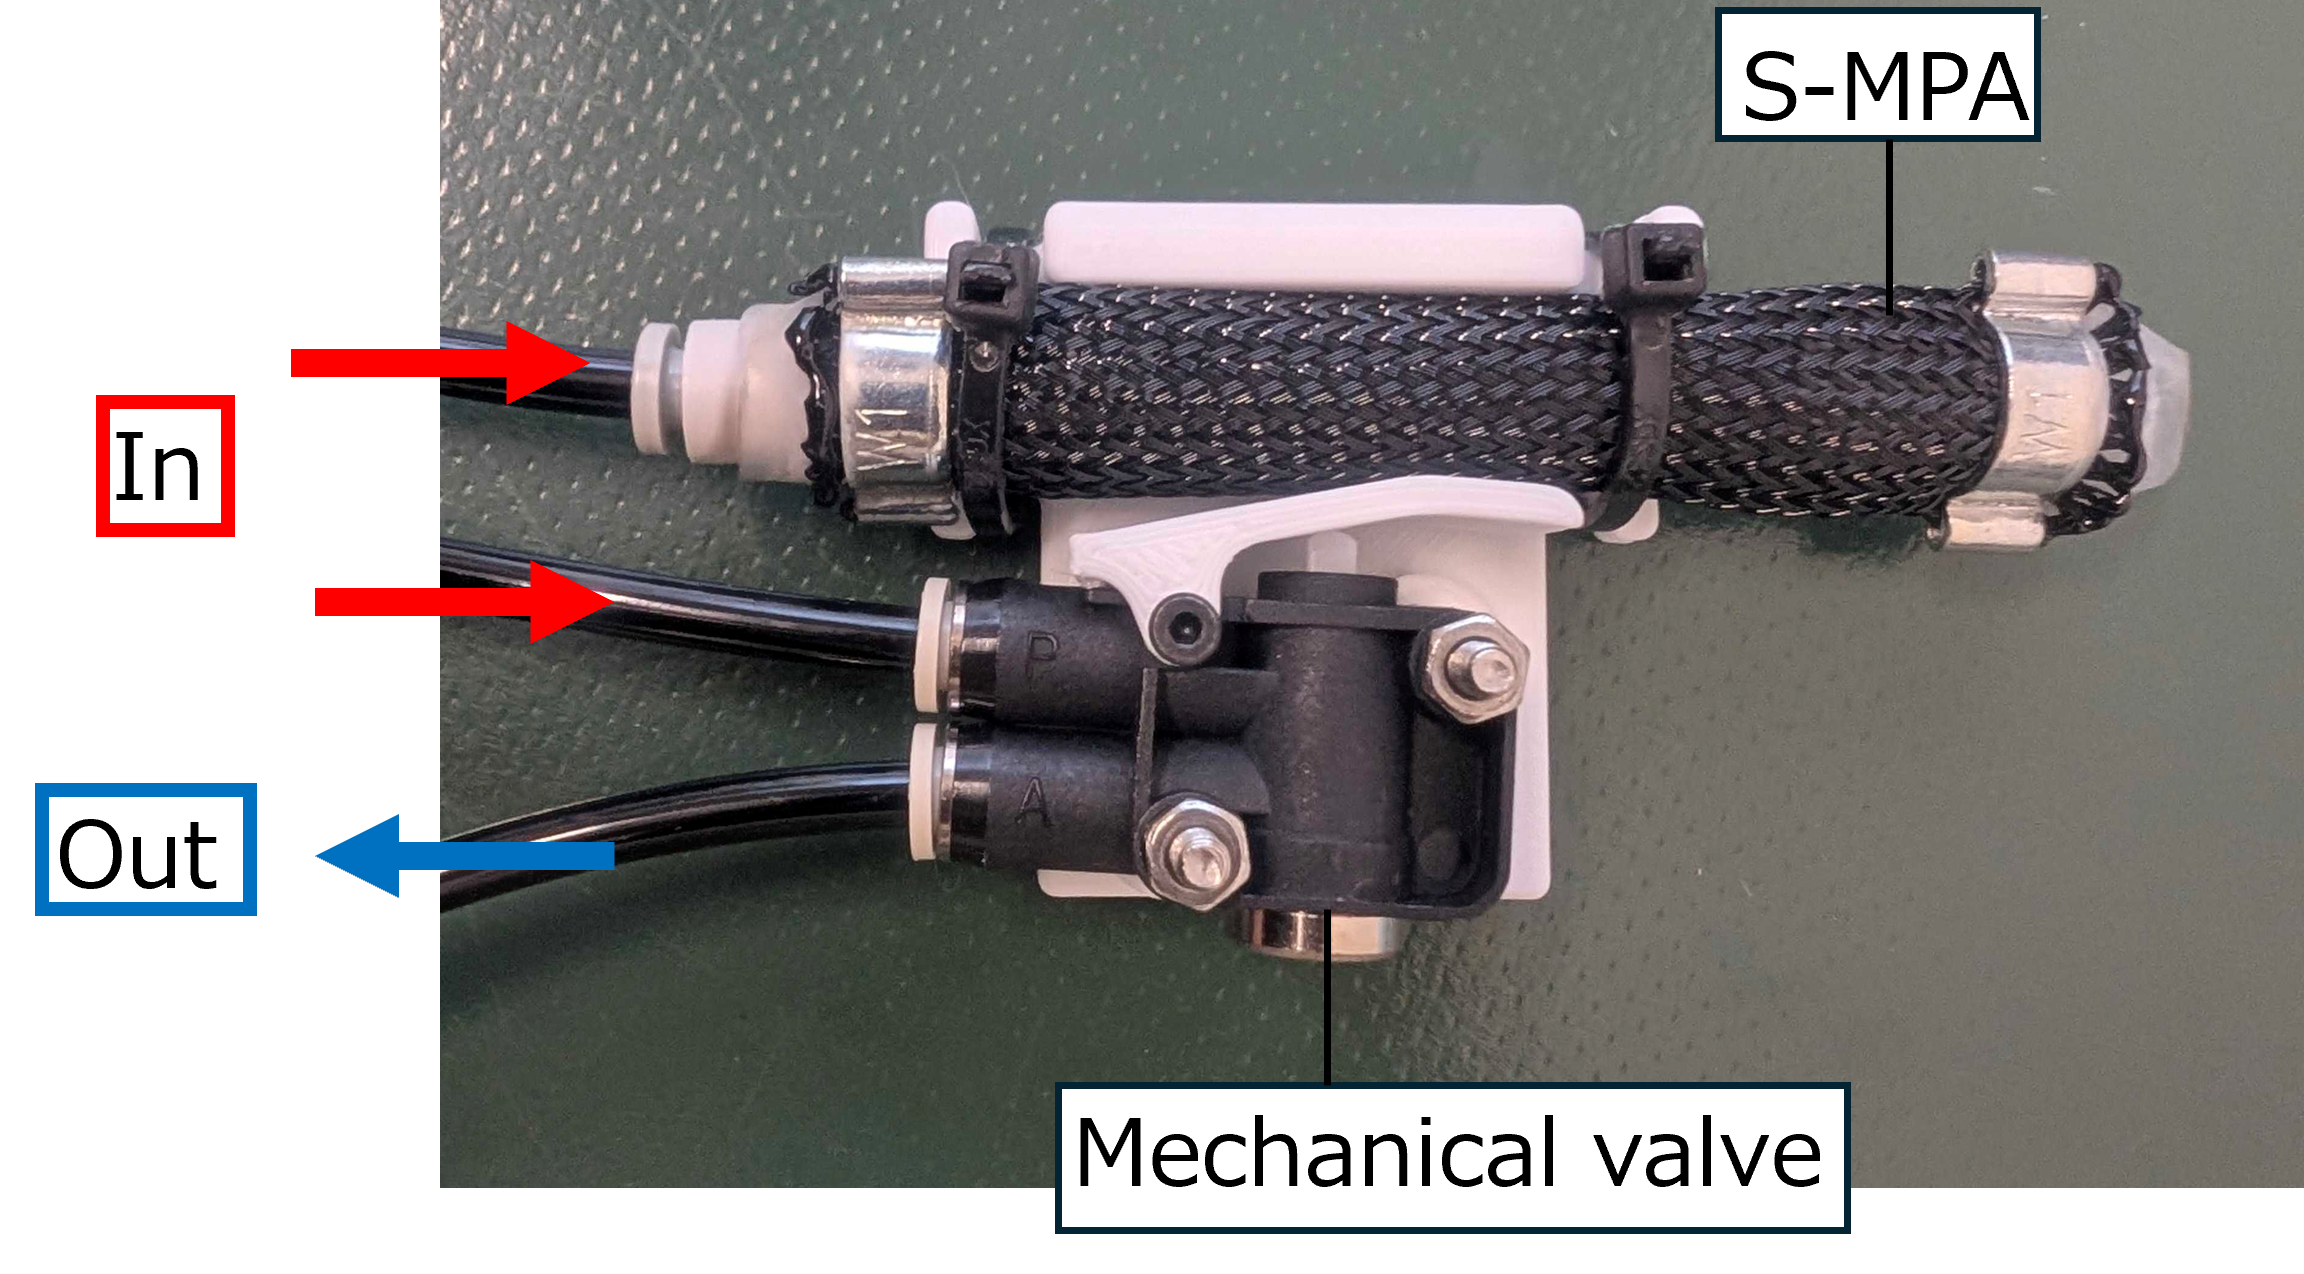
\includegraphics[width=0.45\textwidth]{figure/sensor.png}
    \caption{Appearance of the sensor device used in the pneumatic circuit.}
    \label{fig:sensor_device}
\end{figure}

この自励振動デバイスはメカニカルバルブの種類をNO(ノーマルオープン)とNC(ノーマルクローズ)に変えることで，開閉の条件を反転させることができる．
NOバルブを用いた自励振動デバイスの出力変化の概要をFig.~\ref{fig:sensorsetumei2}に示す．S-PAMが膨張しているときは出力がoffになり，S-PAMが収縮すると出力はonになることで圧縮空気が供給される．
また，NCバルブを用いた自励振動デバイスの出力変化の概要をFig.~\ref{fig:sensorsetumei}に示す．S-PAMが膨張しているときは出力がonになることで圧縮空気が供給され，S-PAMが収縮すると出力はoffになる．これらのメカニカルバルブを用いた自励振動デバイスで，空気圧回路を構成している．
\begin{figure}[t]
    \centering
%    \includegraphics[width=0.5\linewidth]{figure/MPA_moshikizu.png}
    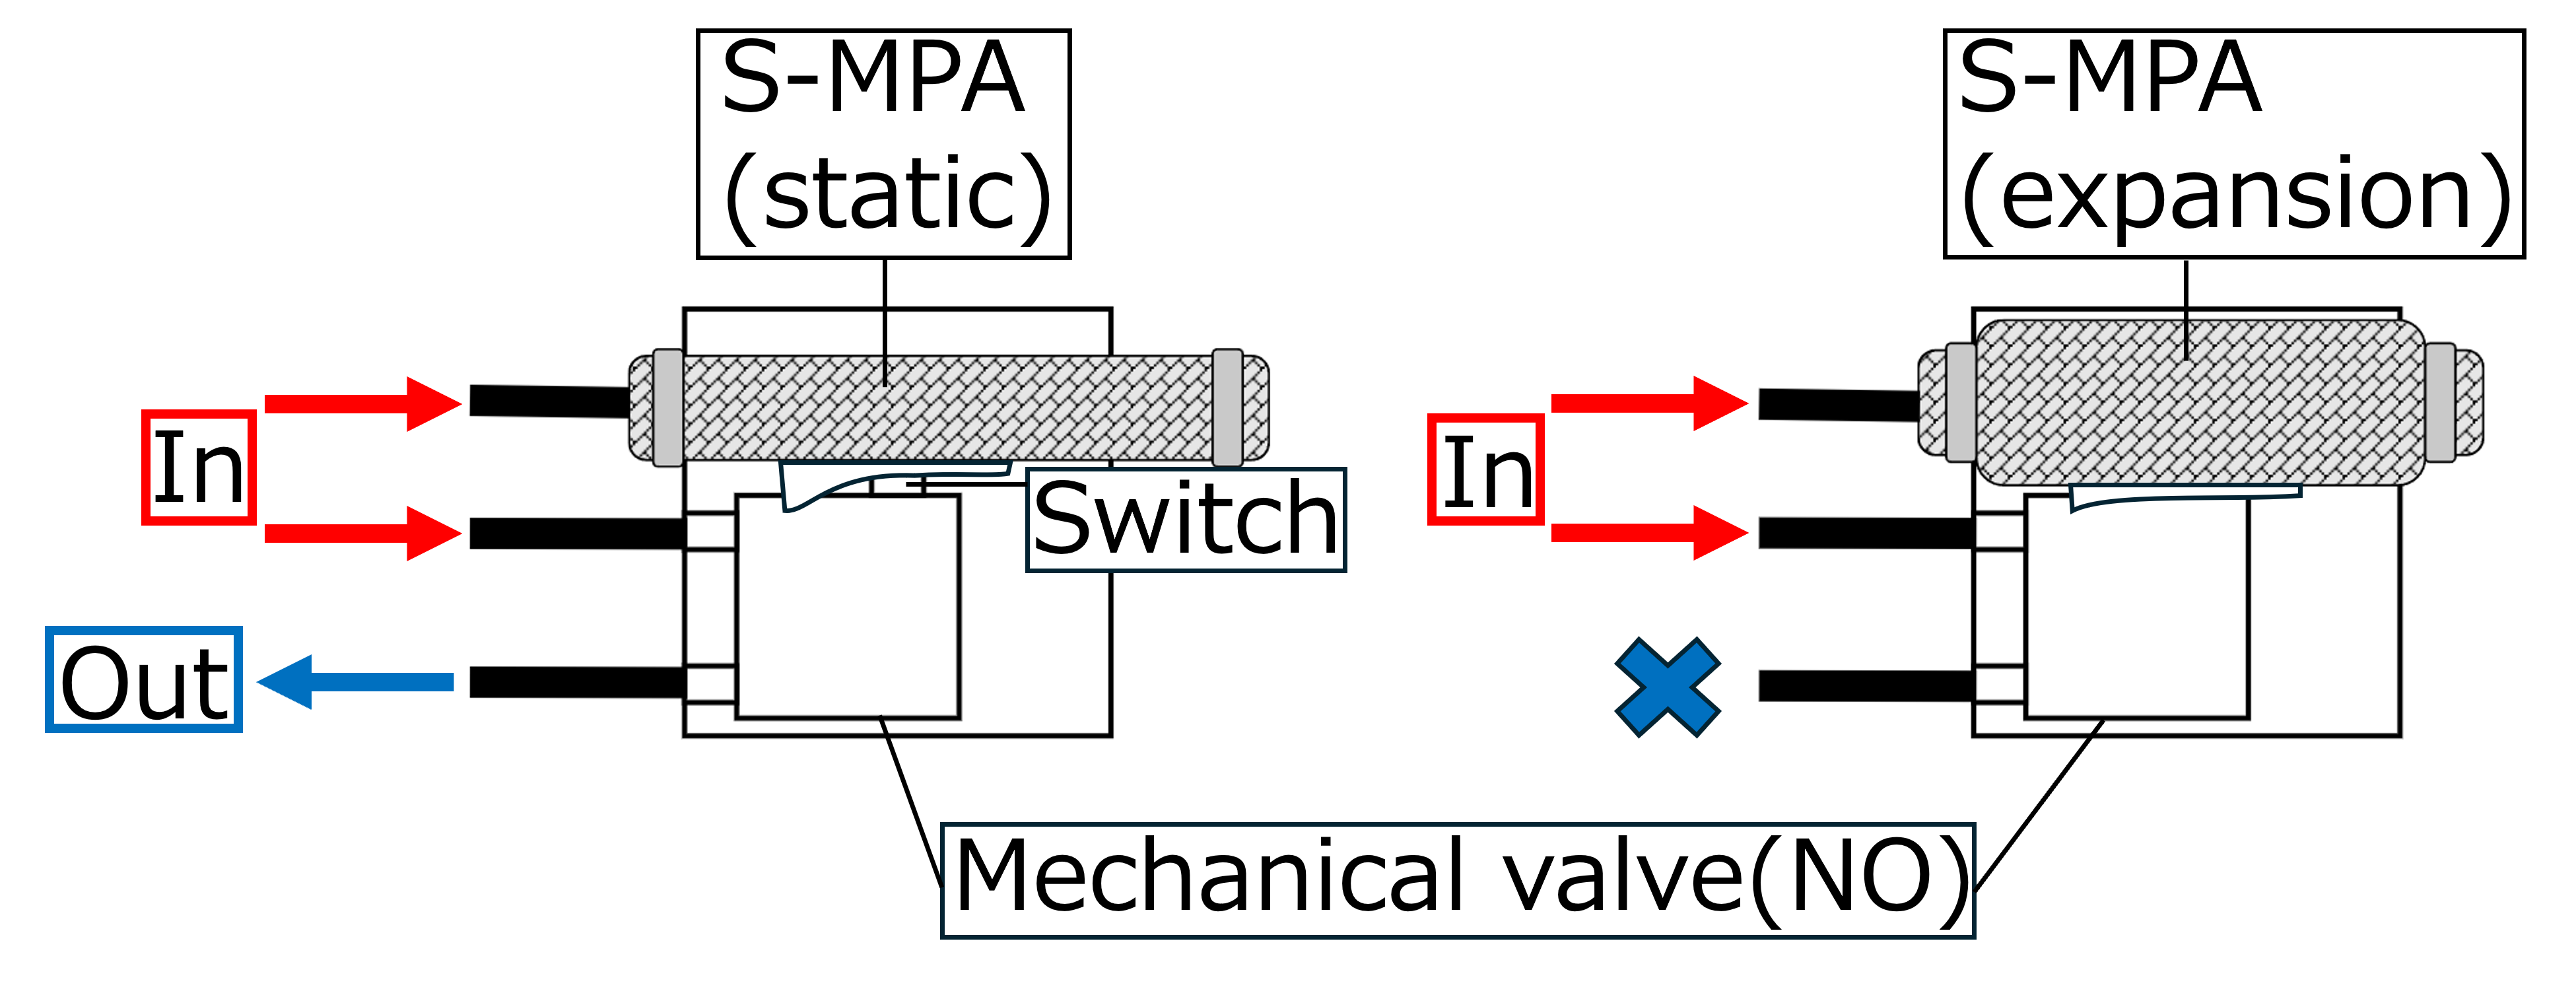
\includegraphics[width=0.45\textwidth]{figure/sensorsetumei2.png}
    \caption{Overview of the output changes of the sensor device using the NO valve.}
    \label{fig:sensorsetumei2}
\end{figure}    
\begin{figure}[t]
    \centering
%    \includegraphics[width=0.5\linewidth]{figure/MPA_moshikizu.png}
    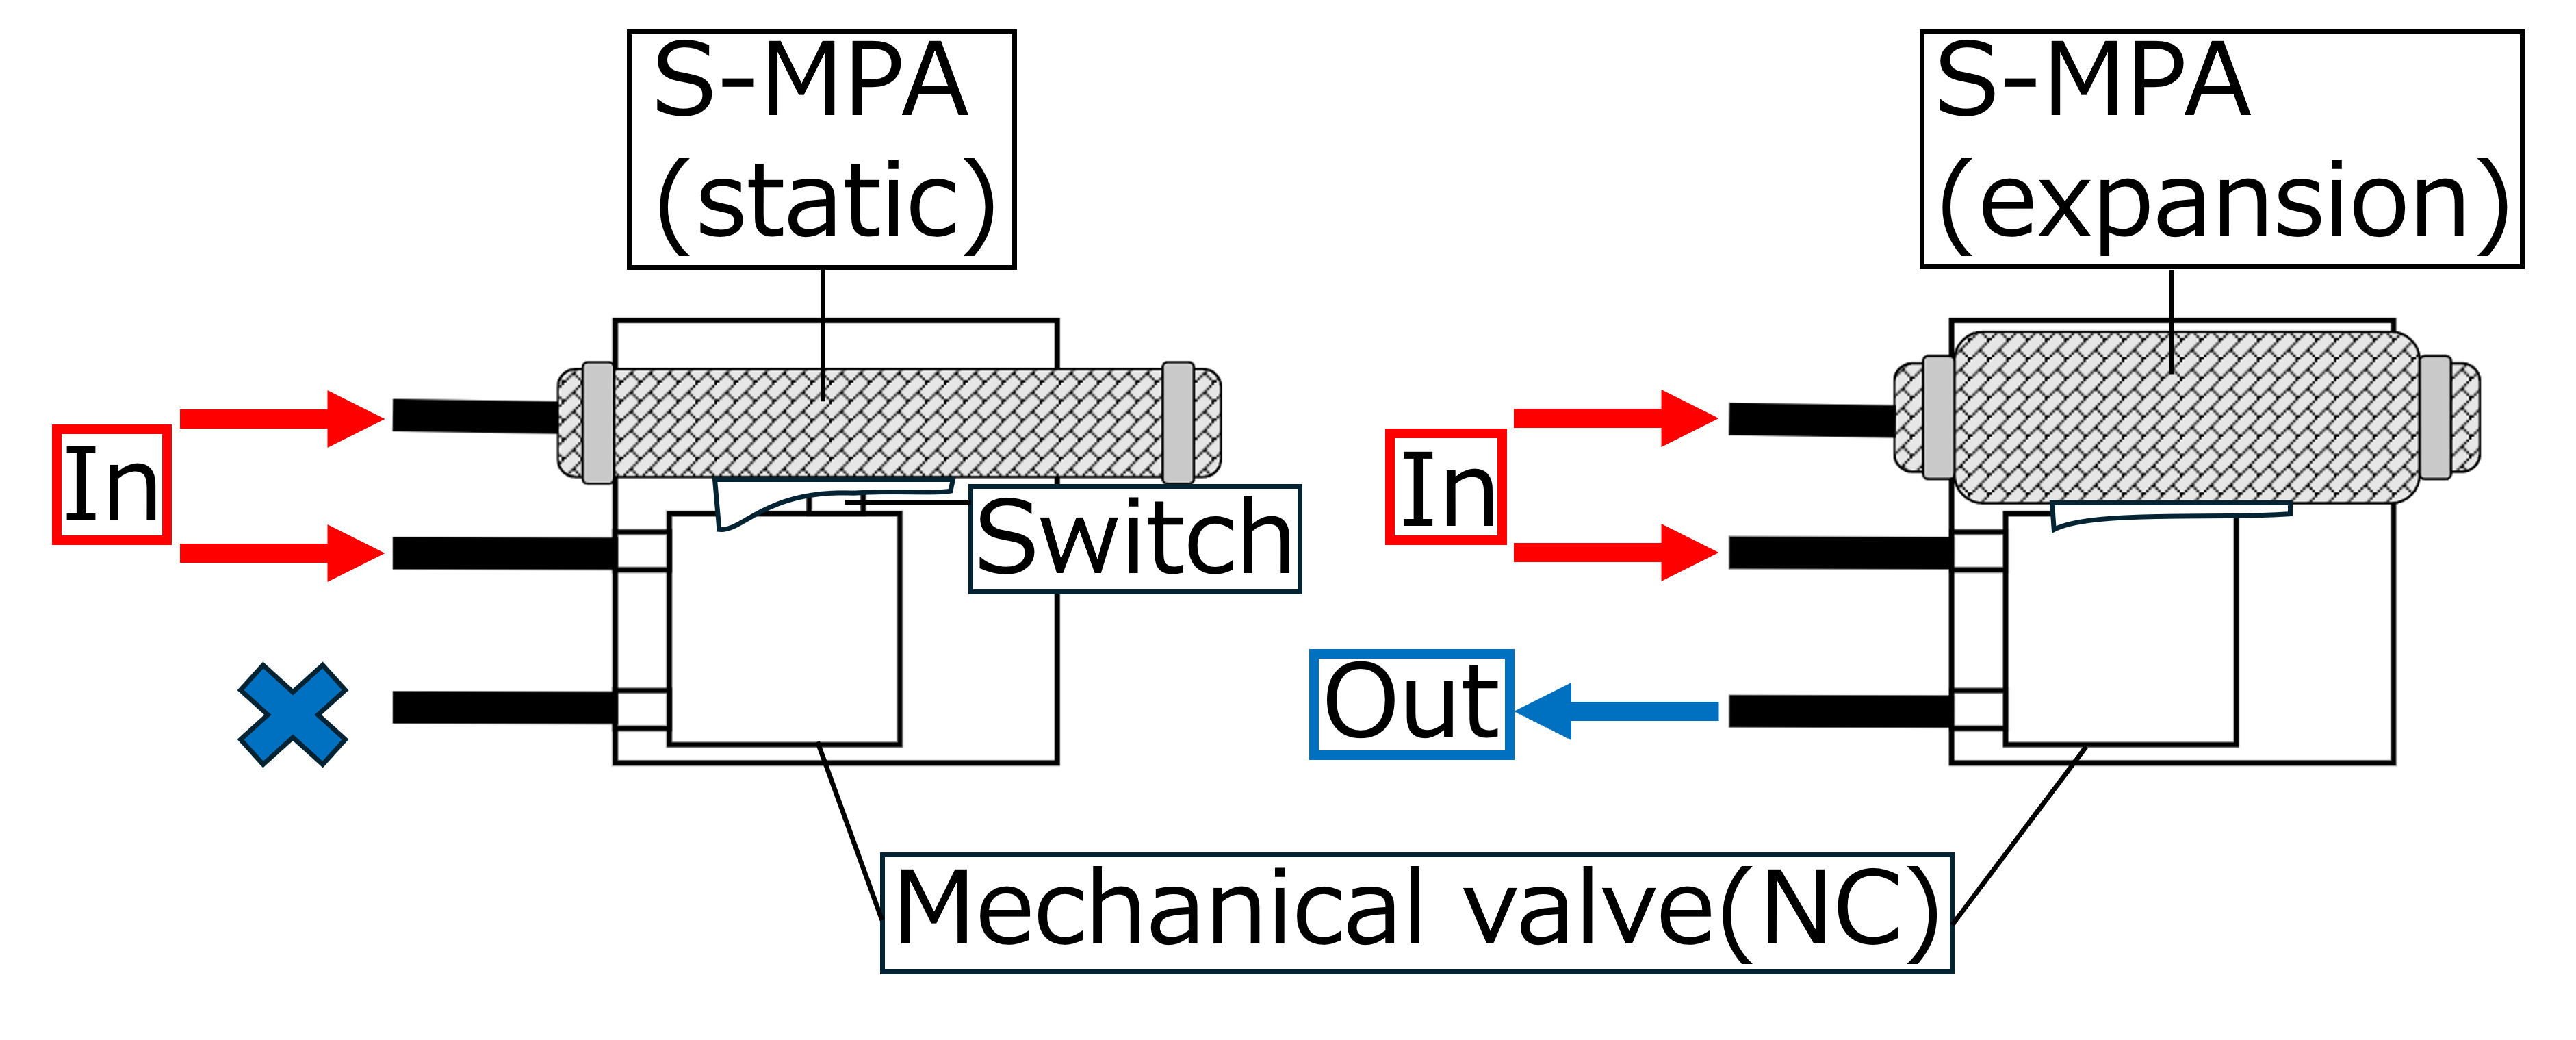
\includegraphics[width=0.45\textwidth]{figure/sensorsetumei.png}
    \caption{Overview of the output changes of the sensor device using the NC valve.}
    \label{fig:sensorsetumei}
\end{figure}

\subsection{空気圧回路の構成}
自励振動デバイスを複数個用いることで空気圧回路を構成している．
NO，NCのメカニカルバルブを用いた自励振動デバイスを組み合わせることで，S-PAMの動きに応じて出力が切り替わり，自励振動(周期運動)を生み出す．
この仕組みを利用して，空気圧回路に接続したA-PAMの収縮および膨張の動きを周期的に変化させ，外力に対応しながら移動するロボットを実現できると考えた．
そこで，まず空気圧回路が生み出す自励振動を確認するために，それぞれの自励振動デバイスを1ユニットずつ組み合わせた，2ユニットの基本構成となる空気圧回路を製作し，Fig.~\ref{fig:air_circuit2}にその外観を示す．
\begin{figure}[t]
    \centering
%    \includegraphics[width=0.5\linewidth]{figure/MPA_moshikizu.png}
    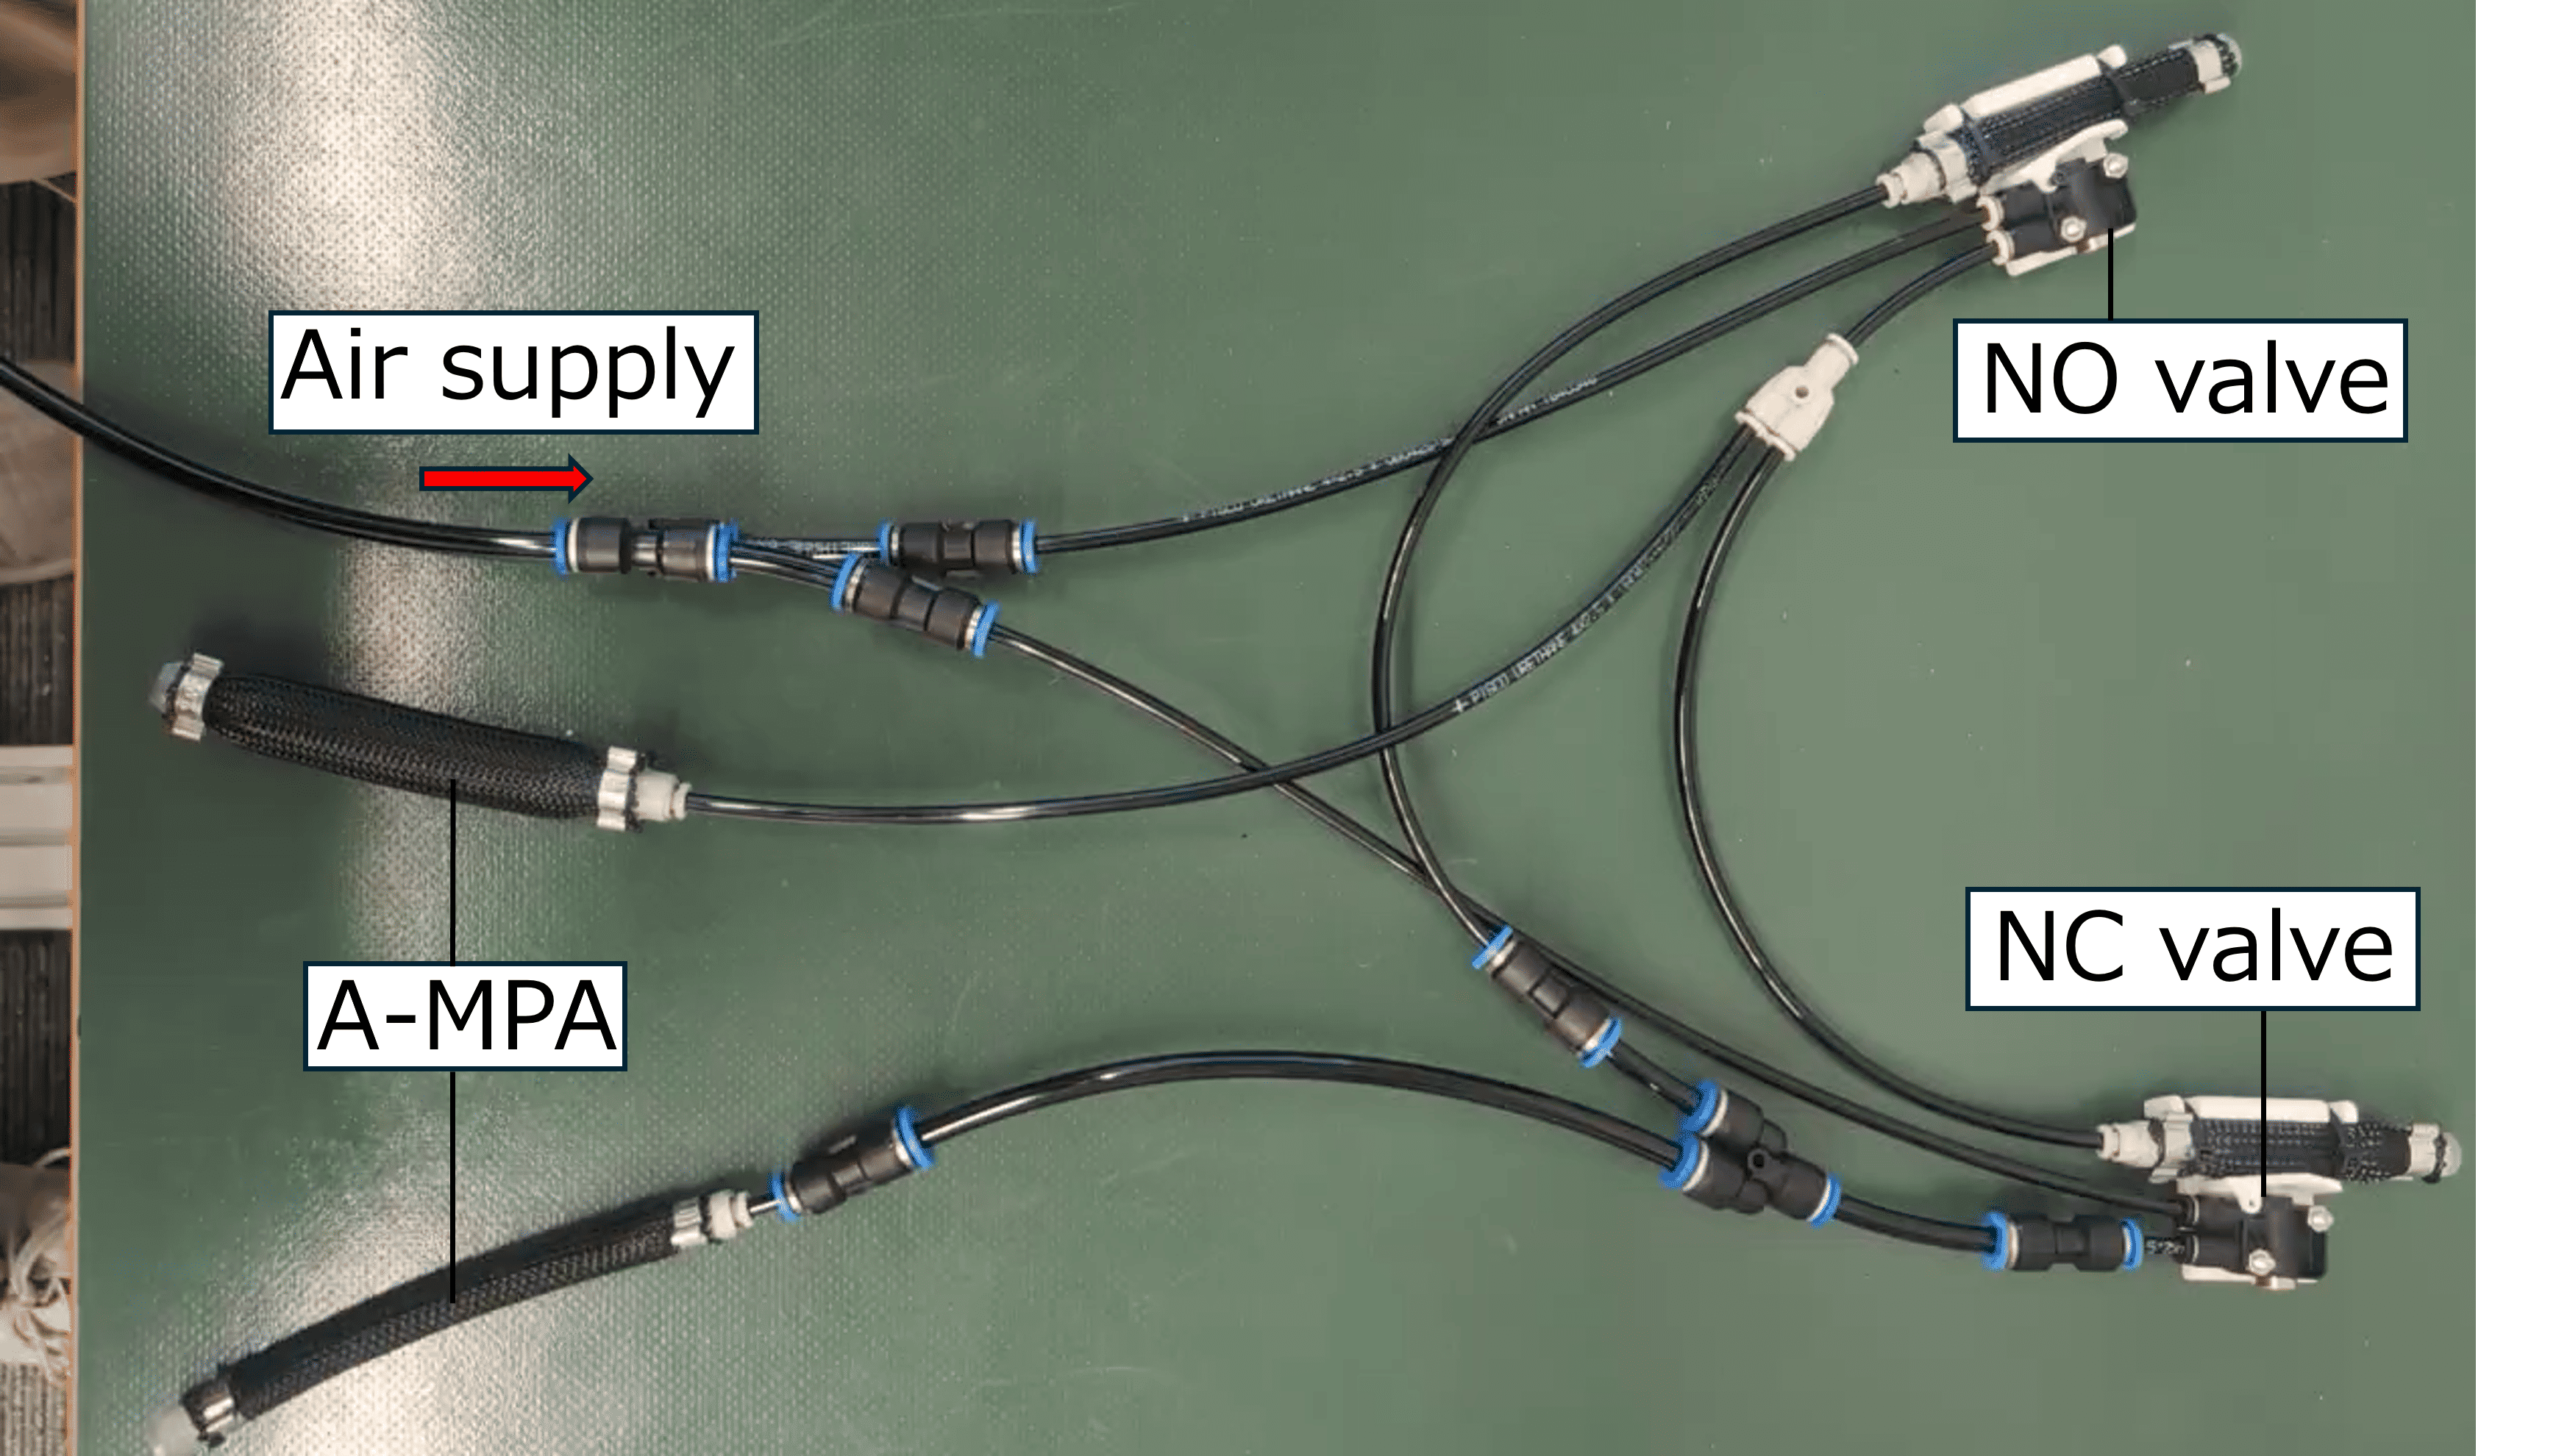
\includegraphics[width=0.45\textwidth]{figure/2unit.png}
    \caption{Appearance of the pneumatic circuit composed of two sensor devices.}
    \label{fig:air_circuit2}
\end{figure}
% 空気圧回路の話をしたい，どのような構成でどのような動きをするのかを説明したい．具体的には，自励振動デバイスがどのような動きをすると，アクチュエータがどのような動きをするのかを説明したい．ただ，前の章で自励振動デバイスの動きを説明しているので，ここでは空気圧回路全体の動きを説明したい．あまり自励振動デバイスの細かい話をせず，空気圧回路全体の動きの説明をしたい．
この空気圧回路は，圧縮空気を印加すると，S-PAMが膨張しているときは出力がoffになり，S-PAMが収縮すると出力がonになるNOバルブを用いた自励振動デバイスと，S-PAMが膨張しているときは出力がonになり，S-PAMが収縮すると出力がoffになるNCバルブを用いた自励振動デバイスとを組み合わせて構成されている．この構成により，各S-PAMの状態に応じて出力が交互に切り替わり，自励振動が生成される．その結果，2つのA-PAMの収縮および膨張の動きは周期的に入れ替わる．


\subsection{A-PAMで構成する脚の概要}
2本のA-PAMを脚軸方向に平行に配置すると，一方が収縮し他方が膨張したときに脚が()する．これにより，空気圧回路が生み出す交互の収縮・膨張を，脚の()として取り出すことができる．
\begin{figure}[t]
    \centering
%    \includegraphics[width=0.5\linewidth]{figure/MPA_moshikizu.png}
    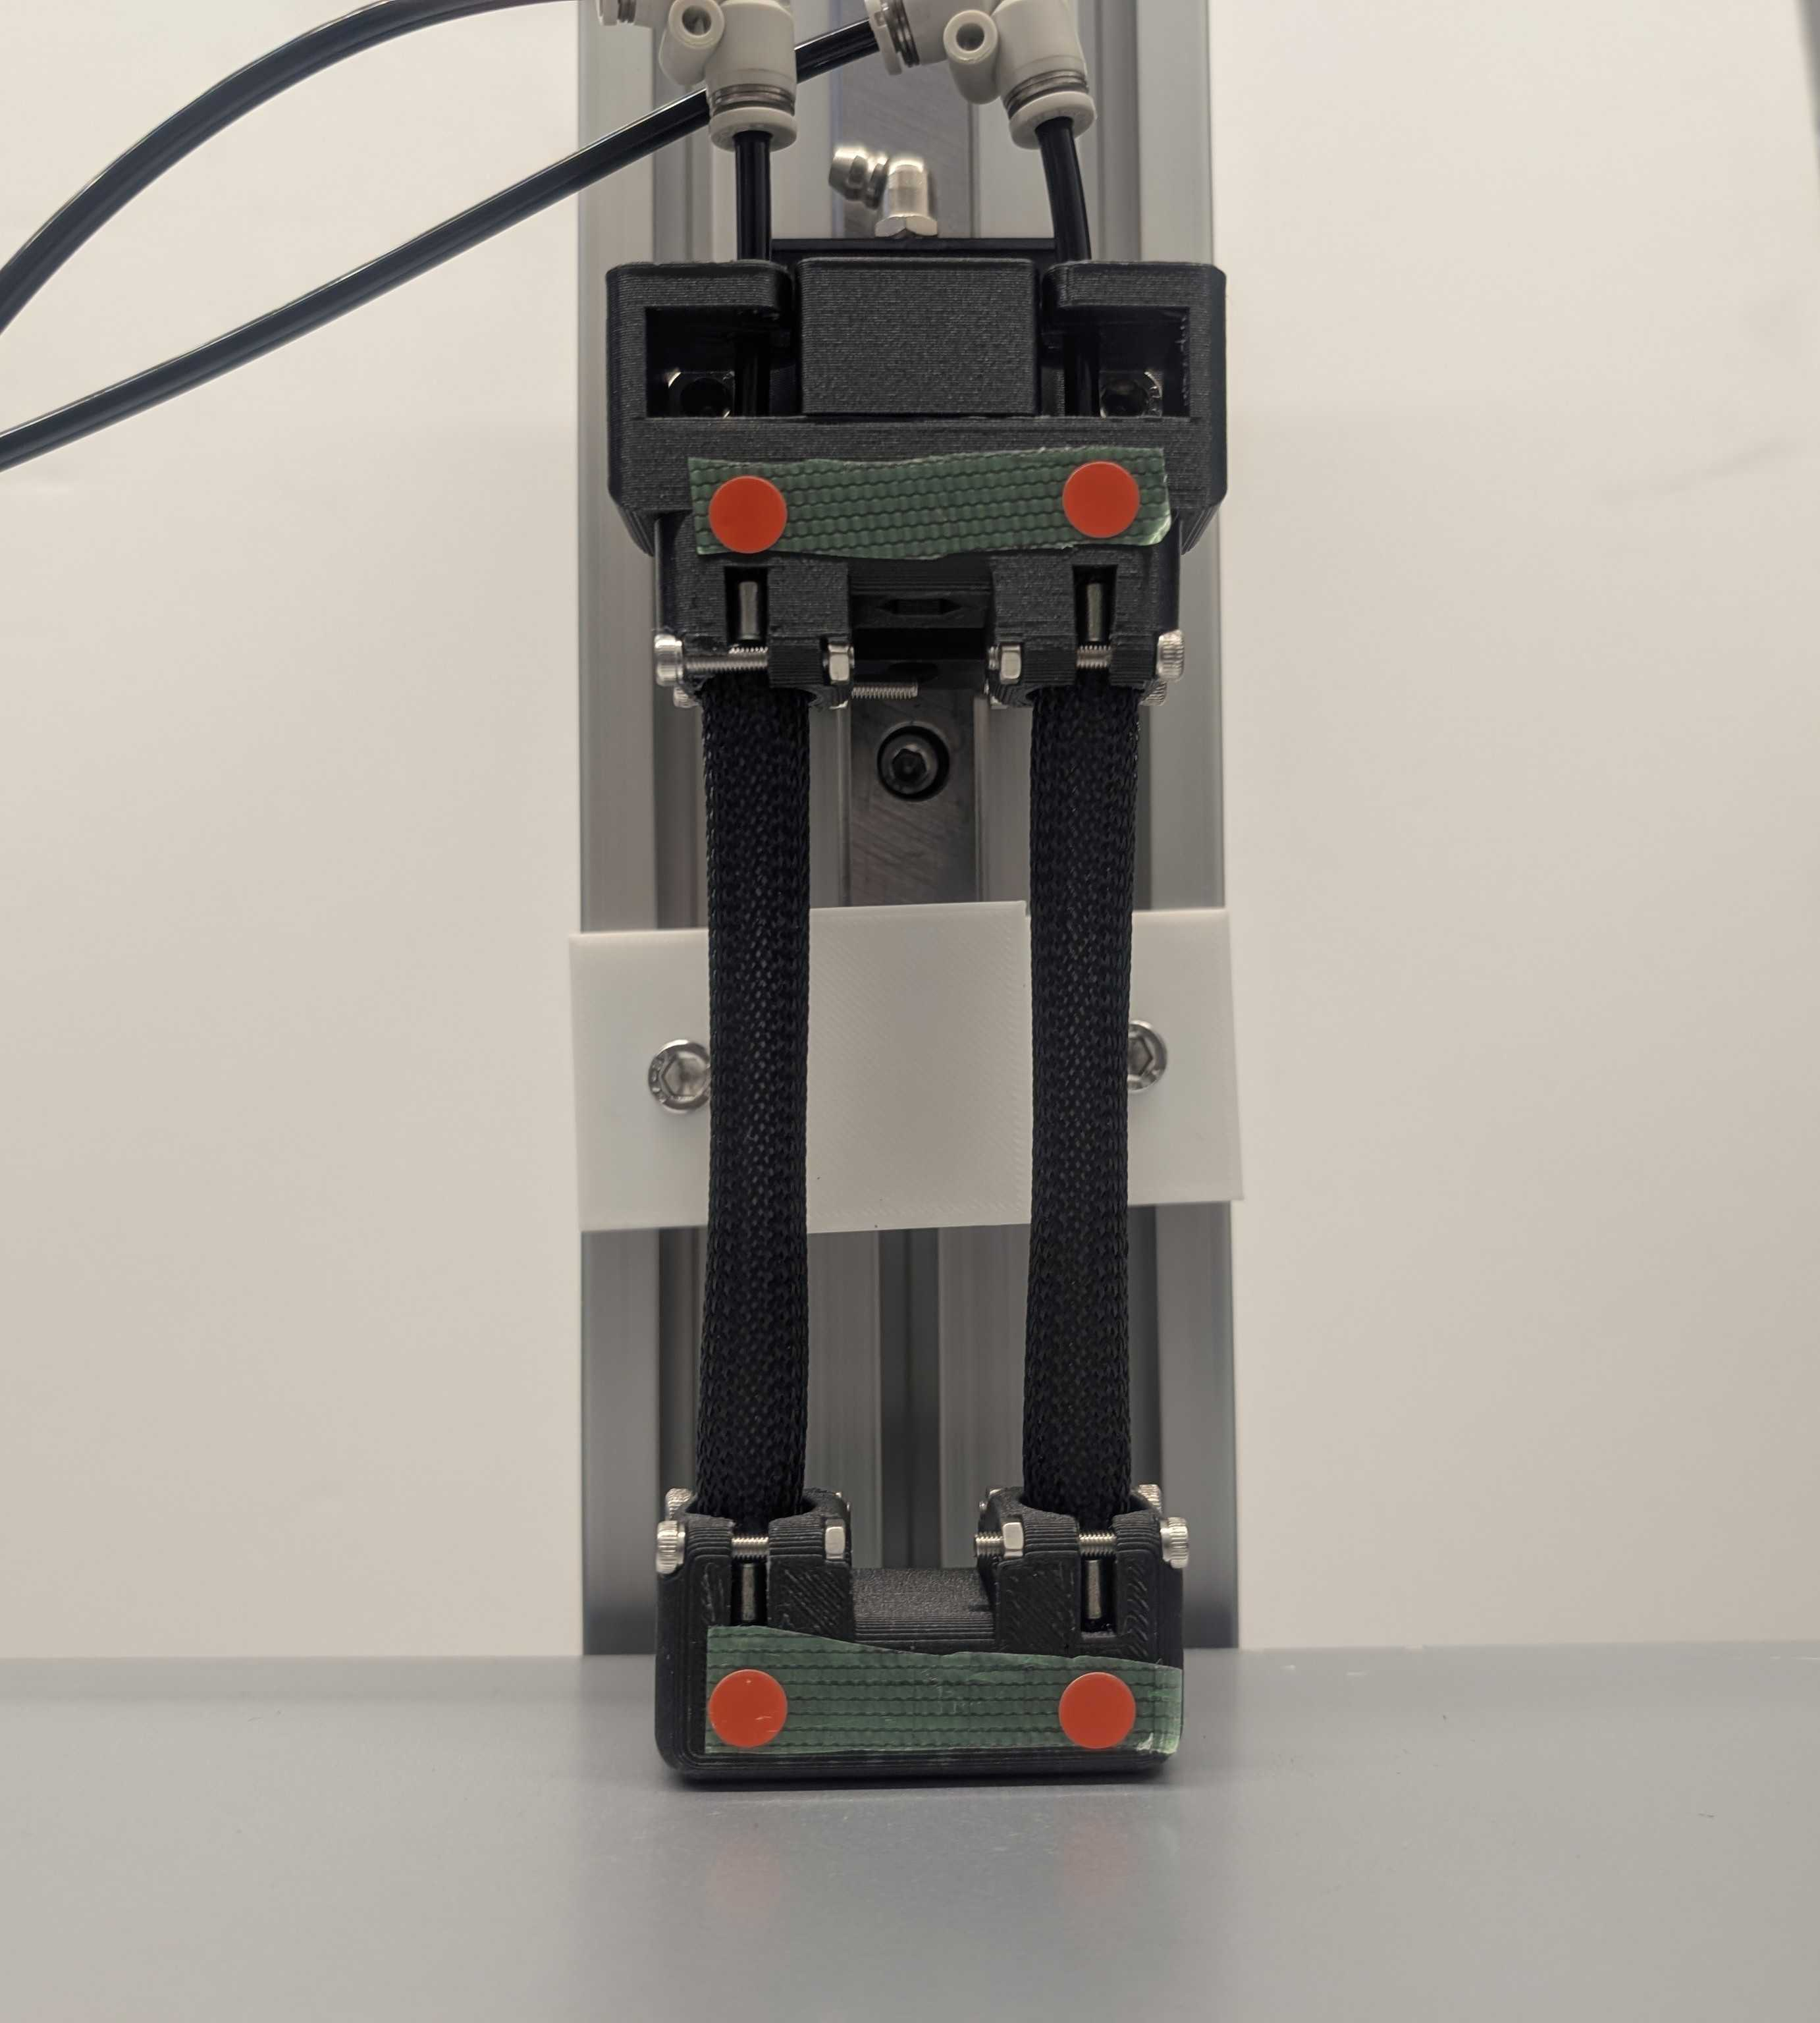
\includegraphics[width=0.45\textwidth]{figure/leg.jpg}
    \caption{Schematic of the leg structure composed of two A-PAMs.}
    \label{fig:leg}
\end{figure}
\section{トラッキングによる脚運動の解析と実験条件について}
本章では，外力による脚運動の変化を解析し，周期運動の変調を明らかにするために，運動を幾何学的に評価できるトラッキング手法を用いた脚運動の解析方法について述べる．また，解析に用いる実験条件についても説明する．
\subsection{脚運動の解析方法}
本実験では，脚の運動を幾何学的に評価するために，トラッキングソフトであるkinoveaを用いる．手法は，脚の運動をカメラで撮影し，画像処理によって脚の位置や角度を抽出することで，脚の運動を定量的に評価することができる．
\subsection{実験条件}
\section{実験結果と今後の取り組み}
本章では現在までに行った研究の進捗と今後の取り組みについて説明する．実験をすることで確認できた周期運動について説明する．
\subsection{実験結果}
\subsection{今後の取り組み}
{\small
%\bibliographystyle{osukalab}
\bibliographystyle{osukalab}
\bibliography{myref}
}

\clearpage

\end{document}

%以下コメント

%ざっと読んだ感じ
% ・全体の構成はいいと思う
% ・細かい言葉遣いや、文献の引用不足(引用すべきところでできていない)、段落間での論理の飛躍が見られるのでこれは後ほど
% ・文章での説明に頼り過ぎていてよくわからない箇所(特に空圧回路の動作機序あたり)があるので、模式図も含めて書いてほしい
% ・目指したいもの(空圧回路でどんなことができればいいか)を緒言でもう少し説明しないと、2章以降のことが大きな目標に対してどうつながっているか分かりづらい。コレはスライドでの説明でも気をつけてほしい
% ・やったことはもっとしっかり説明できた方がよい